\subsection*{Custom loss function}
\begin{frame}
\backupslinklabel{custom_loss}
%\frametitle{Custom loss function for the DNN -- mass range effect}

\begin{minipage}[c]{.475\textwidth}
\only<1>{\begin{center}\vspace{-4pt}
\begin{tikzpicture}%
\node[anchor=south west,inner sep=0] at (0,0) {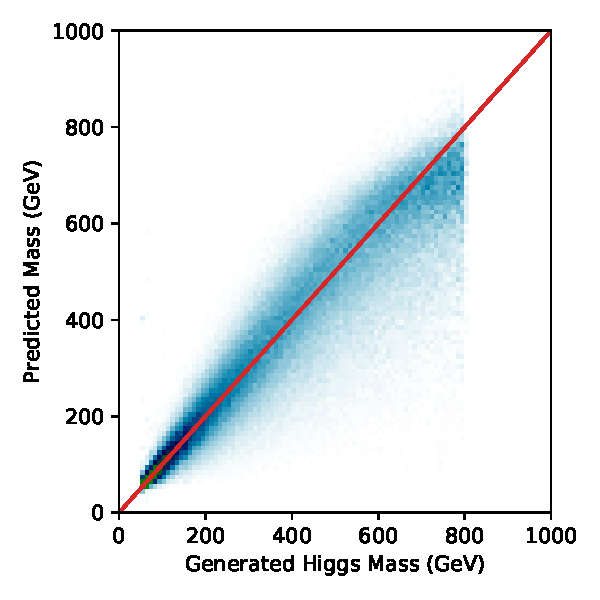
\includegraphics[height=\graphh]{\PhDthesisdir/plots_and_images/my_plots/ML/from_ML_plots/DNNs_for_discussion/Mass_range/predicted_vs_answers_histo-NN-activation-softplus-batch_size-2048-mape-Adam-gu-inclusive-3-layers-1000-neurons-en.pdf}};

\draw [ltcolororange, thick] (2.45, 1.1) -- (2.45, 6.7);
\draw [ltcolororange, thick] (3.985, 1.1) -- (3.985, 6.7);

\draw [ltcolorviolet, thick] (1.5, 2.2) -- (6.5, 2.2);
\draw [ltcolorviolet, thick] (1.5, 3.9) -- (6.5, 3.9);

\end{tikzpicture}
\end{center}}
\only<2>{
\manip {\color{ltcolorred} How to cope with the boundaries?}
\submanip Bias to be balanced,
\submanip Extend the mass range?
\subsubmanip Would be nice!
\subsubmanip Not always feasible...

\manip Every horizontal slice is one predicted value:
\submanip \og Same family \fg{} of events to the NN.
%\submanip Actually $\sim$ centered on the red line!
%\subsubmanip {\footnotesize Center of the distributions in the red rectangles.}
}

\only<3>{\begin{center}\vspace{-4pt}
\begin{tikzpicture}%
\node[anchor=south west,inner sep=0] at (0,0) {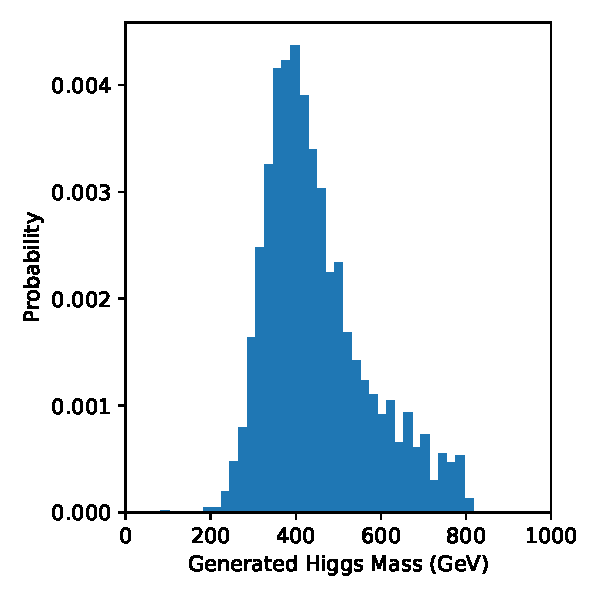
\includegraphics[height=\graphh]{\PhDthesisdir/plots_and_images/my_plots/ML/from_ML_plots/DNNs_for_discussion/Mass_range/distributions/distribution-inclusive-Higgs_mass_gen-at_pred_mass_400weighted-is_test-en.pdf}};

\draw (6.5, 6) node [left] {\small $\sim$ Symmetric \OK};
\end{tikzpicture}
\end{center}}
\only<4>{\begin{center}\vspace{-4pt}
\begin{tikzpicture}%
\node[anchor=south west,inner sep=0] at (0,0) {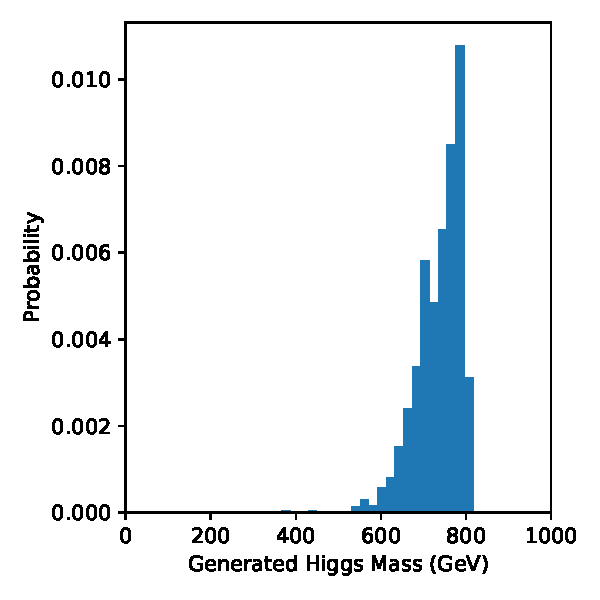
\includegraphics[height=\graphh]{\PhDthesisdir/plots_and_images/my_plots/ML/from_ML_plots/DNNs_for_discussion/Mass_range/distributions/distribution-inclusive-Higgs_mass_gen-at_pred_mass_750weighted-is_test-en.pdf}};

\draw (1.5, 6) node [right] {\small Cropped distribution!};
\draw (1.5, 5.25) node [right] {\small Only low mass tail is here:};
\draw (1.5, 4.25) node [right, text width=3.5cm] {\scriptsize With full distribution, the DNN would have learnt to predict higher values};
\end{tikzpicture}
\end{center}}
\end{minipage}
\hfill
\begin{minipage}[c]{.475\textwidth}
\begin{center}\vspace{-4pt}
\begin{tikzpicture}
\node[anchor=south west,inner sep=0] at (0,0) {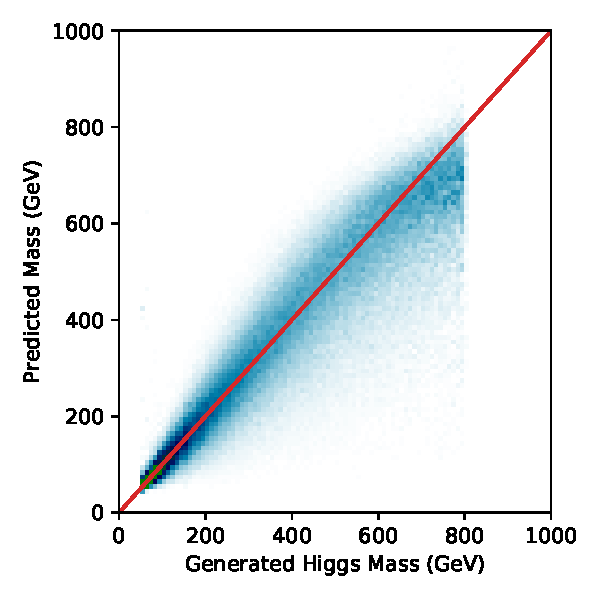
\includegraphics[height=\graphh]{\PhDthesisdir/plots_and_images/my_plots/ML/from_ML_plots/trained_NNs_FastSim/DeepTau-inclusive/PuppiMET_with_METcov_j1j2jr_Nnu_Npu/predicted_vs_answers_histo-NN-ADAM_glorot_uniform-activation-softplus-batch_size-2048-mape-Adadelta-u-inclusive-3-layers-1000-neurons-en.pdf}};

\only<1>{
\draw [ltcolororange, thick] (1.675, 1.1) -- (1.675, 6.7);
\draw [ltcolororange, thick] (5.55, 1.1) -- (5.55, 6.7);

\draw [ltcolorviolet, thick] (1.5, 1.3) -- (6.5, 1.3);
\draw [ltcolorviolet, thick] (1.5, 5.65) -- (6.5, 5.65);
}

\only<3>{
\draw [ltcolorred, thick] (1.5, 3.25) rectangle (5.55, 3.4);
\draw (2.25, 1.5) node [right] {\small Events at \SI{400}{\GeV} to the NN};
\draw [-latex, ltcolorgreen, thick] (4.25, 1.7) to[in=-45, out=60] (3.75, 3.2);
}

\only<4>{
\draw [ltcolorred, thick] (1.5, 5.25) rectangle (5.55, 5.4);
\draw (2, 6.3) node [right] {\small Events at \SI{750}{\GeV} to the NN};
\draw [-latex, ltcolorgreen, thick] (2.6, 6.1) to[in=135, out=-120] (3, 5.5);
}

\end{tikzpicture}
\end{center}\vspace{-5pt}
\end{minipage}

\end{frame}

\begin{frame}
\begin{minipage}[c]{.475\textwidth}
\begin{center}\vspace{-4pt}
\begin{tikzpicture}%
\node[anchor=south west,inner sep=0] at (0,0) {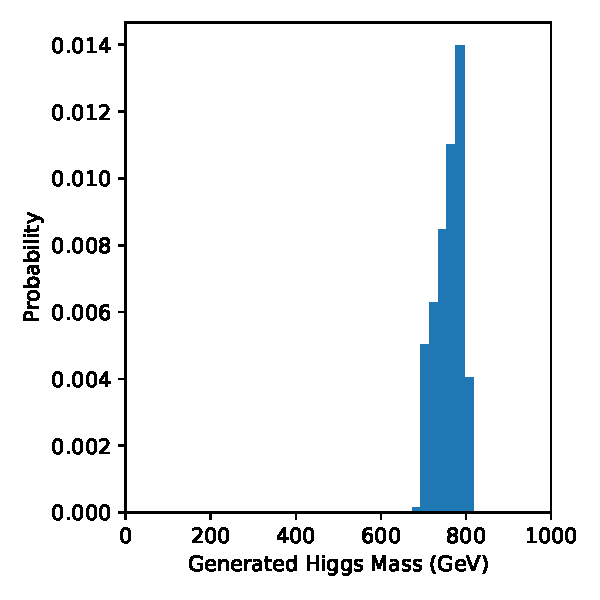
\includegraphics[height=\graphh]{\PhDthesisdir/plots_and_images/my_plots/ML/from_ML_plots/DNNs_for_discussion/Mass_range/distributions/distribution-inclusive-Higgs_mass_gen-mirrored_cut_at_pred_mass_750weighted-is_test-en.pdf}};

\draw (1.5, 6) node [right] {\small Crop again, restore symmetry};
\end{tikzpicture}
\end{center}
\end{minipage}
\hfill
\begin{minipage}[c]{.475\textwidth}
\begin{center}\vspace{-4pt}
\includegraphics[height=\graphh]{\PhDthesisdir/plots_and_images/my_plots/ML/custom_loss-illustrations/distance_and_mirror-en.tex}
\end{center}\vspace{-5pt}
\end{minipage}
\end{frame}


\begin{frame}

\begin{minipage}[c]{.51\textwidth}
\begin{align*}
\LossMAPEsqrtb(\ytrue, \ypred)
&=
\LossMAPEsqrt(\ytrue, \ypred)
\\&
\times
\left\lbrace
\begin{aligned}
0 \quad & \text{if $(\ytrue, \ypred)\in$ area 3}\\
\num{0.1} \quad & \text{if $(\ytrue, \ypred)\in$ area 4}\\
1 \quad & \text{else}
\end{aligned}
\right.
\end{align*}
\begin{align*}
\LossMAPEsqrt(\ytrue, \ypred)
&=
\LossMAPE(\ytrue, \ypred) \times \sqrt{\ytrue}
\\&=
\abs{\frac{\ypred-\ytrue}{\ytrue}} \times \sqrt{\ytrue}
\nonumber\\\Leftrightarrow
\LossMAPEsqrt(\ytrue, \ypred)
&=
\abs{\frac{\ypred-\ytrue}{\sqrt{\ytrue}}}
\mend
\end{align*}
\end{minipage}
\hfill
\begin{minipage}[c]{.475\textwidth}
\begin{center}\vspace{-4pt}
\includegraphics[height=\graphh]{\PhDthesisdir/plots_and_images/my_plots/ML/custom_loss-illustrations/areas-EN.tex}
\end{center}\vspace{-5pt}
\end{minipage}

\end{frame}